\documentclass[a4paper, 12pt]{article}
\usepackage{graphicx}
\usepackage[utf8]{inputenc}
\usepackage[ukrainian]{babel}
\usepackage{amsmath}
\usepackage{fancyhdr}
\usepackage{geometry}
\geometry{top=2cm, bottom=2cm, left=3cm, right=1.5cm}
\usepackage[colorlinks=true,linkcolor=blue]{hyperref}%
\begin{document}

\begin{titlepage}
	\begin{center}
		\Large
		\textbf{Київський національний університет імені Тараса Шевченка} \\
		Факультет комп'ютерних наук та кібернетики \\

		\vspace{6cm}

		\textbf{\LARGE ЗВІТ ДО ЛАБОРАТОРНОЇ РОБОТИ №3} \\[0.5cm]
		\textbf{З дисципліни ``Чисельні методи''} \\[0.5cm]
		\textbf{Тема: Розв'язування системи нелінійних алгебраїчних рівнянь} \\

		\vfill
		\hspace{7cm} Виконав студент 3-го курсу \\
		\hspace{7cm} групи ТТП-31 \\
		\hspace{7cm} Рісенгін Владислав \\
		\vspace{2cm}

		Київ-2024
	\end{center}
\end{titlepage}

\newpage

\hbadness=99999

\section{Постановка задачі}

Придумати систему яка складається з 3 нелінійних рівнянь. І вектором правої частини $\vec f = (0, 0, 0)$. \\

Розв'язати її методом простої ітерації, і модифікованим методом Ньютона

\section{Вступ}

Метою цієї лабораторної роботи є вивчення методів розв'язування системи нелінійних алгебраїчних рівнянь, 
які дають можливість вирішення багатьох наукових та інженерних задач. \\

У процесі виконання роботи будуть досліджені та реалізовані методи простої ітерації, модифікований метод Нютона.

\section{Деталі реалізації}

Лабораторна робота виконана використовуючи мову програмування Python, а також бібліотеку numpy.

\clearpage
\section{Теоретичний опис методів}
% \subsection{Метод простої ітерації}

\begin{figure}[ht]
	\centering
	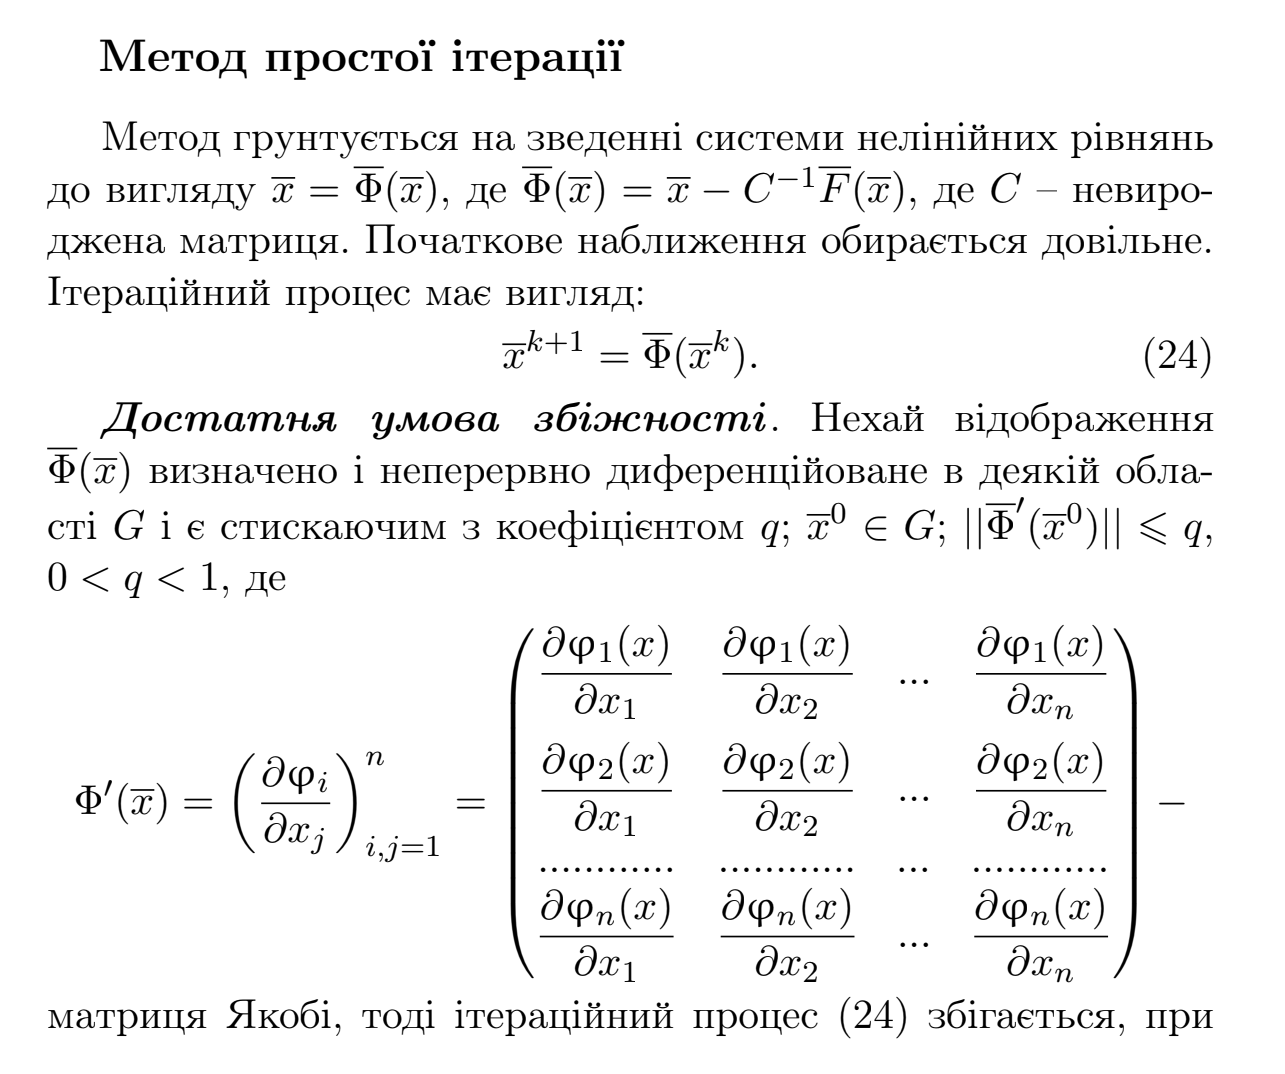
\includegraphics[width=0.9\linewidth]{iteration1.png}
\end{figure}
\begin{figure}[ht]
	\centering
	
\includegraphics[width=0.9\linewidth]{iteration2.png}
\end{figure}

\clearpage
\newpage
% \subsection{Модифікований метод Ньютона}

\begin{figure}[ht]
	\centering
	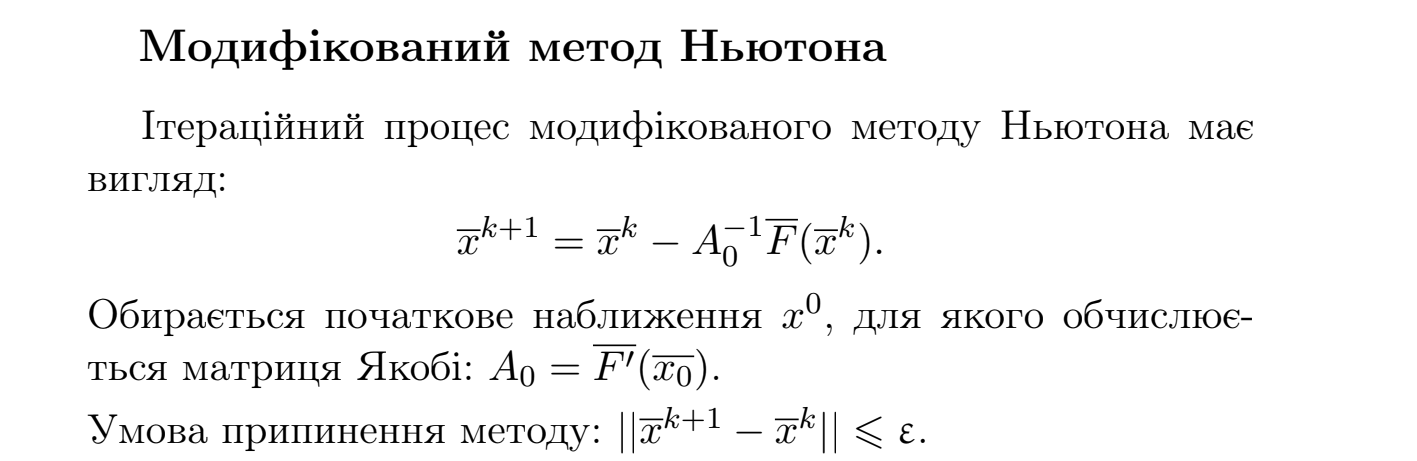
\includegraphics[width=0.9\linewidth]{mod_nuton1.png}
\end{figure}

\newpage

\section{Результати роботи програми}

Для обох методів будемо шукати розв'язок з точністю $\epsilon < 10^{-6}$ \\
Як критерій зупинки використовується норма $max(|x_1|, |x_2|, ..., |x_n|) < \epsilon$ \\ 
Система для розв'язання: 
\[
\begin{cases}
3x_1 - \sin(x_2) - \frac{1}{e^{x_3}} = 0 \\
5x_2 + \cos(x_1) - x_3^2 = 0 \\
4x_3 + x_1^2 - x_2 = 0
\end{cases}
\]

\subsection{Метод простої ітерації}

\begin{verbatim}
Iteration  |                  x_new                   |    Norm   
----------------------------------------------------------------------
0          | [0 0 0]                                  | -
1          | [ 0.333333 -0.200000  0.000000]          | 0.333333333
2          | [ 0.267110 -0.188991 -0.077778]          | 0.077777778
3          | [ 0.297671 -0.191698 -0.065085]          | 0.030561143
4          | [ 0.292241 -0.190357 -0.070076]          | 0.005430095
5          | [ 0.294460 -0.190538 -0.068941]          | 0.002218911
6          | [ 0.293995 -0.190441 -0.069311]          | 0.000465066
7          | [ 0.294159 -0.190458 -0.069219]          | 0.000164057
8          | [ 0.294121 -0.190451 -0.069247]          | 0.000038556
9          | [ 0.294133 -0.190452 -0.069239]          | 0.000012384
10         | [ 0.294130 -0.190452 -0.069242]          | 0.000003121
11         | [ 0.294131 -0.190452 -0.069241]          | 0.000000948
\end{verbatim}

Збіжність досягнута після 11 ітерацій. Остаточний розв'язок:
\[
x = [ 0.29413083, -0.19045207, -0.06924108]
\]

Перевірка результату:
\[
f(\text{x}) = [ 7.47620013e-07, -1.93551788e-07,  6.78223201e-07]
\]

\subsection{Модифікований метод Ньютона}

\begin{verbatim}
Iteration  |                  x_new                   |    Norm   
----------------------------------------------------------------------
0          | [0 0 0]                                  | -
1          | [ 0.283333 -0.200000 -0.050000]          | 0.283333333
2          | [ 0.293009 -0.191526 -0.067951]          | 0.017950890
3          | [ 0.294027 -0.190552 -0.069102]          | 0.001150762
4          | [ 0.294120 -0.190462 -0.069228]          | 0.000126747
5          | [ 0.294130 -0.190453 -0.069240]          | 0.000011542
6          | [ 0.294131 -0.190452 -0.069241]          | 0.000001154
7          | [ 0.294131 -0.190452 -0.069241]          | 0.000000110
\end{verbatim}

Збіжність досягнута після 7 ітерацій. Остаточний розв'язок:
\[
x = [ 0.29413063, -0.19045205, -0.06924121]
\]

Перевірка результату:
\[
f(\text{x}) = [-6.40065623e-09, -4.05407964e-08,  5.12418141e-08]
\]

\newpage
\section{Висновок}

У результаті роботи обох методів було досягнуто розв'язку з необхідною точністю \(\epsilon < 10^{-6}\). \\ 

Метод простої ітерації виявився менш ефективним, потребуючи 11 ітерацій для досягнення збіжності. \\ 
Остаточний розв'язок: \(x = [0.29413083, -0.19045207, -0.06924108]\) пройшов перевірку, показавши значення функцій, близькі до нуля, що свідчить про правильність розв'язку. \\ 

З іншого боку, модифікований метод Ньютона виявився значно швидшим, досягнувши збіжності вже за 7 ітерацій. \\ 
Остаточний розв'язок: \(x = [0.29413063, -0.19045205, -0.06924121]\) також продемонстрував малі значення функцій у цій точці, підтверджуючи його коректність. \\ 

Отже, можна стверджувати, що модифікований метод Ньютона є більш ефективним у даному випадку, забезпечуючи швидшу збіжність і високу точність розв'язку в порівнянні з методом простої ітерації. \\ 

Це підкреслює важливість вибору відповідних чисельних методів для розв'язання нелінійних систем рівнянь, залежно від їхніх властивостей та вимог до точності.

\end{document}
